\chapter{ Realidad aumentada sin marcadores }

\section{Aspectos técnicos}
\subsection{Descripción}
La realidad aumentada es una tecnología que permite entremezclar el mundo virtual con el mundo, añadiendo la información virtual a la información física ya existente en tiempo real, permitiendo al usuario comprender mejor el entorno que le rodea. Hace unos pocos años, con la aparición de los dispositivos móviles más potentes y las librerías gratuitas de realidad aumentada, el desarrollo de esta tecnología se ha vuelto muy accesible para cualquier desarrollador. Esto implica un aumento drástico en el número de ideas y aplicaciones que se generan cada día con el paso de los años.\\

En la actualidad existen tres tipos de realidad aumentada:
\begin{itemize}
\item \textbf{Realidad aumentada con marcadores (2D y 3D)}: Los marcadores pueden ser imágenes impresas o dibujos en los que la aplicación reconoce el marcador y activa la experiencia sobre dicho marcador.
\item \textbf{Realidad aumentada sin marcadores}: Esta es la tecnología más novedosa, ya que combina diferentes tecnologías como (SLAM, seguimiento del movimiento, reconocimiento del ambiente, detección de planos ...) para proyectar el objeto y mantenerlo en el mismo punto de anclaje sin ayuda de ningún marcador.
\item \textbf{Realidad aumentada por geolocalización}: Este tipo de experiencias vinculan a la RA con una ubicación geolocalizada específica. Normalmente se utilizan en exteriores y proporcionan información contextual sobre el ambiente que nos rodea.
\end{itemize}
Las posibilidades de la realidad aumentada sin marcadores están en pleno auge y cada vez aparecen más aplicaciones que mejoran la experiencia de usuario y facilitan el trabajo en algunos sectores como puede ser la fábrica, la arquitectura, la medicina, la educación y muchos más.

\subsection{Métodos de tracking}
El \textit{tracking} es como conocemos al proceso de localización espacial del usuario en un entorno. Es uno de los aspectos clave en el desarrollo de aplicaciones de realidad aumentada ya que cuanto mejor sea la estimación de la posición y orientación del dispositivo sensor, mejores y más acertados serán los resultados y la inmersión por parte del usuario.\cite{BostanciTrackingMethods}\\

El cálculo del \textit{tracking} se encarga de posicionar la cámara relativamente a los objetos de la escena. Existen multitud de tecnologías y métodos para llevarlos a cabo, siendo los más comunes sensores mecánicos, magnéticos, sónicos, dinámicos y basados en visión. Éstos últimos son los más extendidos, ya que la mayoría de los dispositivos desde los que se despliegan las aplicaciones de realidad aumentada, como móviles o tablets, disponen de una o varias cámaras. \cite{ARToolkit}\\

El \textit{tracking} basado en cámaras de visión es un subcampo del \textit{tracking} 3D, en el que se utilizan algoritmos de visión por ordenador para obtener de la manera más precisa posible el posicionamiento de seis grados de libertad del dispositivo (tres grados de posición y otros tres de orientación).\\

En este tipo de posicionamiento es necesario disponer de un conjunto de marcadores o referencias tridimensionales para situar la cámara con respecto a ellas. Aunque recientemente se ha tendido a utilizar en menor medida los marcadores físicos para dar una experiencia más rápida y cómoda al usuario, han sido una herramienta imprescindible en los primeros pasos de la realidad aumentada para la obtención de la localización relativa de la cámara.
Según David Marimón\cite{TrackingThesis}, fundador y director general de Catchoom, se pueden distinguir dos aproximaciones distintas a la hora del tracking: los métodos Bottom-Up y los Top-Down. 

\subsubsection{Bottom-Up}
Las aproximaciones del tipo Bottom-Up pretenden obtener la posición del dispositivo basándose en la información que recibe a través de la cámara.
Para este método de tracking la posición y orientación se calculan en base a la obtención de características geométricas de objetos y sus relaciones. Dependiendo de los datos procesados, el seguimiento puede ser con marcas o sin ellas.\\
El tracking basado en marcas era el método más extendido en los inicios de la realidad aumentada. Hace sus cálculos con la ayuda de marcadores físicos que en su mayoría presentan un gran contraste entre blanco y negro para que los sensores puedan percibirlos con mayor facilidad. Existen también marcadores que usan códigos de colores y diferentes formas geométricas, aunque después de ser sometidos a prueba se comprobó que los más sólidos eran los marcadores cuadrados. Por otra parte, este método es especialmente sensible a la oclusión, ya que cuando se pierde el marcador, es imposible calcular la posición del dispositivo. Por este motivo, se han diseñado marcadores que puedan hacer frente a este problema con imágenes en escala de grises que completan marcas que no son visibles.\\
Paralelamente, el \textit{tracking} sin marcas se basa únicamente en las características intrínsecas de la escena, estructuras físicas de fácil percepción como las esquinas de una mesa.\\
Existen técnicas en este campo que utilizan información sobre superficies planas detectadas en el campo de visión, siendo su principal inconveniente su alto coste computacional (actualmente este tipo de localización no lo pueden llevar a cabo todos los dispositivos del mercado).\\
Por otra parte, hay técnicas basadas en modelos. No están considerados marcadores porque son parte del medio natural, pero al igual que con éstos los cálculos se basan en el reconocimiento de los objetos que existen y que el programa está preparado para procesar.\\
Finalmente, existen métodos que actúan en escenarios donde no se es capaz de obtener planos o modelos. Se suelen emplear restricciones epipolares de las cámaras en movimiento. Sin embargo, esta técnica no es utilizada habitualmente por sus altos requisitos de cómputo.\\
\subsubsection{Top-Down}
Las aproximaciones del tipo Top-Down intentan estimar desde la posición actual del dispositivo si se está percibiendo lo que se esperaba. Es decir, primero se estima la posición y después se confirma esa estimación con los datos del medio.
En este caso, se emplean modelos del movimiento basados en filtros bayesianos para hacer una predicción de la localización del dispositivo. Partiendo de esta estimación, se busca mediante la cámara una serie de referencias parciales que corrijan la predicción y mejoren el posicionamiento del observador. Por ello, todos los modelos Top-Down se ven obligados a trabajar con filtros y modelos de asociación de datos.
El uso de estos filtros permite combinar varios métodos de tracking y mantener un registro constante de los objetos y la cámara, aunque los marcadores, modelos o planos sean parcialmente visibles por oclusión o se hayan escapado del campo de visión.
Además del seguimiento óptico, se han desarrollado numerosas alternativas con las que proporcionar otros métodos de localización (como los beacons o la ubicación del GPS) y así complementar y facilitar una localización más precisa y correcta. A las aproximaciones que se valen de varias de estas técnicas se las denomina métodos de fusión.

\subsection{Tecnologías implicadas en la RA sin marcadores}
El objetivo de la realidad aumentada es integrar contenido virtual en el mundo real. Idealmente, dicho contenido se tendría que comportar exactamente como uno real, esto requiere una información muy precisa sobre la posición del dispositivo que usa el usuario con respecto al objeto virtual. Para ello, se han desarrollado diferentes tecnologías que junto a los sensores de los teléfonos actuales (giroscopio, acelerómetro, sensor de luz) y a la cámara, permiten disfrutar de una experiencia casi ideal. \cite{ARCarmigniani} 

\subsubsection{SLAM(Simultaneuos localization and mapping)}
Mapeo y localización simultáneos se le llama a la tecnología que se basa en una serie de algoritmos complejos que utiliza los datos de los sensores para construir un mapa de un entorno desconocido y a su vez para saber dónde está localizado el dispositivo. Esta técnica es usada por robots y por vehículos autónomos. 
¿Cuál es el objetivo? Descubrir donde estoy. La tecnología SLAM, en el momento que empieza el algoritmo, no tiene ningún tipo de información del entorno. Normalmente, sólo tarda unos pocos segundos en crear un mapa aproximado del entorno con lo que calcula una posición inicial. Más adelante, el mapa creado va creciendo y mejorando en base a la información que obtiene desde el fotograma de la cámara.
Aunque este término empezó a aparecer en la década de los 90, las primeras implementaciones carecían de cámaras o sensores que proporcionaban información visual. En 2005 comenzó a abaratarse el coste de los ordenadores y de las cámaras, y los investigadores empezaron a combinar el SLAM con sensores visuales. Hasta este punto, esta tecnología estaba pensada para la navegación con robots en entornos desconocidos, hasta que en 2007 Georg Klein y David Murray vieron el potencial de usar esta tecnología en la realidad aumentada. \cite{MaxstMedium}

\subsubsection{Reconocimiento del ambiente}
Cuanto mejor entienda la aplicación como es el entorno que le rodea, mejor será la experiencia de usuario. En este apartado, también entra el reconocimiento de superficies, tanto horizontales como verticales. El funcionamiento de esta tecnología consiste en procesar cada fotograma obtenido por la cámara y encontrar puntos característicos, estos puntos pueden ser cualquier cosa que ayuden a identificar objetos (esquinas, líneas, bordes de objetos, colores, gradientes, etc…), por lo que si se intenta detectar un plano en una superficie donde el color sea uniforme, y carezca de textura o patrones, como puede ser una pared totalmente blanca, seguramente no funcione con normalidad \cite{ARCoreConcepts}. Con estos puntos, luego se construye una maya que va a servir como superficie en la escena de nuestra aplicación y con la cual podremos interactuar activándole las físicas y colisión.
\subsubsection{Estimación de la luz}
Esta tecnología es muy importante ya que aporta un nivel de detalle excelente, los modelos 3D virtuales se comportan como si fueran reales, se iluminan con la iluminación del mundo físico y emiten sombras. La estimación de la luz es posible gracias a la combinación de la información del seguimiento del movimiento y usando un algoritmo de análisis de imagen que determina la intensidad de la luz en la imagen del dispositivo. Cuanto más se mueva la cámara y más información recoja sobre el entorno, más precisos serán los datos de dónde viene la mayor fuente de luz, analizando el nivel de brillo de los píxeles de los fotogramas, por lo que se puede estimar la dirección en la que viene. A esta información se puede acceder desde Unity o el motor que se use, donde se le aplican los valores obtenidos a una la luz posicional.
\subsubsection{Oclusión}
El término oclusión se refiere a cuando un objeto nos impide ver otro objeto o imagen que hay detrás. Para disfrutar de una experiencia de realidad aumentada realista, esta tecnología es esencial, los objetos virtuales tienen que seguir esta regla, porque en el momento en el que cruza una persona delante del objeto, o cruzas la esquina, y sigues viendo el objeto virtual, se arruina la inmersión que podemos llegar a tener. Por lo que no sirve únicamente saber dónde está situado nuestro dispositivo con respecto al objeto, si no también hace falta saber si hay otro objeto o superficie en medio.\cite{articleOclusion}
\subsubsection{Detección de rostros}

Uno de los puntos más importantes de la realidad aumentada en la actualidad es la detección de caras y su reconocimiento.\\

Cada cara está compuesta por al menos 80 rasgos distinguibles, como la distancia que existe entre los extremos de la mandíbula, la profundidad de las cuencas oculares o la separación que hay entre los agujeros de la nariz. \cite{BBC_FacialRecognition}Los humanos somos especialmente buenos reconociendo estos rasgos porque tenemos una zona del cerebro dedicada específicamente a interiorizar patrones.
Basándonos en el funcionamiento del cerebro de una persona hemos desarrollado algoritmos que imitan estas asociaciones, dividiendo las caras en un conjunto de puntos de referencia a los que llamamos nodal points y buscando correspondencias con otras fotos tomadas anteriormente. El algoritmo que sigue un sistema para tratar de identificar si lo que está viendo es una cara pasa por comprobar si existe en la imagen un patrón similar al que formarían normalmente los rasgos más característicos de una cara, para después preguntarse de quién es esa cara. Sin embargo, no existen dos fotos de una misma persona que sean iguales, de manera que los algoritmos tienen que lidiar con 4 problemas fundamentales a la hora de reconocer la cara de una persona: el envejecimiento, la pose, la iluminación y las emociones.\\

En los últimos años se ha desarrollado un sistema de reconocimiento en 3D llamado Deepface, que es capaz de tomar una foto en 2D de un individuo y crear un modelo tridimensional. De esta forma, el sistema tendrá muestras de los rasgos faciales desde todos los ángulos disponibles, solucionando así el problema de la pose.\\

Por otra parte, el problema del envejecimiento también ha sido debidamente prevenido, ya que al crear la estructura 3D de la cara se tienen en cuenta los nodal points más importantes y que menos varían con el transcurso de los años, como son las curvas de los ojos, de la nariz o de la barbilla. Pero lo que realmente ha supuesto un avance en este campo es el Deep Learning, que es un sistema de algoritmos que guía al programa redirigiéndole si va por mal camino. Cada vez que asocia una cara correcta o incorrectamente, registra el proceso por el que ha pasado para realizar la comprobación y queda guardado en un mapa que va ampliándose sucesivamente con cada acierto o error del sistema. De esta manera, cuantas más conexiones se creen mayor será la fiabilidad a la hora de reconocer una cara.\\

Facebook por ejemplo se vale de este método para el reconocimiento facial y posee una red neuronal de más de 20 millones de nodos, con una fiabilidad del 97.35 \%(datos de 2015)\cite{Facebook_FacialRecognition} y que aun así es inferior a la capacidad de detección de una persona.\\\

Se espera que con la mejora de la tecnología el reconocimiento facial sea una forma de identificación tan válida como las huellas dactilares y que puedan identificarse las caras de las personas incluso en grabaciones de seguridad en calidad baja y sin color, así como un método de reconocer el género, edad y otras características del individuo para ofrecerle un servicio o producto más acorde con él en ámbitos como la publicidad.\\
\begin{figure}[H]
     \centering
     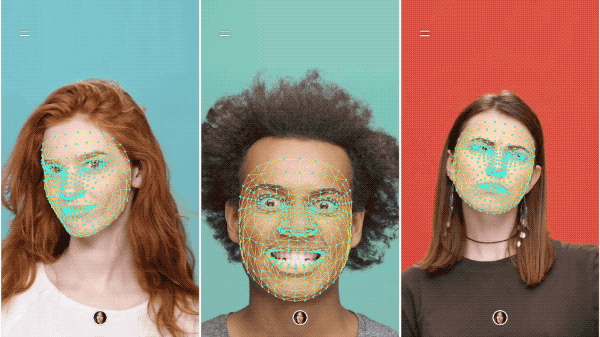
\includegraphics[width=0.7\textwidth]{Images/FaceRecognition.png}
     \caption{Detección de rostros}
     \label{fig:FaceRecognition}
 \end{figure}

\subsubsection{Puntos de ancla en la nube (Cloud Anchor)}
El Cloud Anchor es un mecanismo que permite a los usuarios de una aplicación de realidad aumentada añadir objetos virtuales a una escena. De esta manera múltiples usuarios pueden interactuar y ver los mismos objetos desde dispositivos distintos, pero compartiendo un mismo espacio físico. Su funcionamiento es muy similar al de los anchors comunes, que se utilizan para fijar un objeto en una posición, con la diferencia de que los Cloud Anchors se hospedan en los servidores de Google. De esta manera varios dispositivos pueden consultarlos para situar los objetos en la aplicación.\\

Para ser utilizados, la aplicación en cuestión tiene que tener conexión a internet.
Los Cloud Anchors son actualmente propios del SDK de ARCore, están soportados tanto en Android como en iOS (siempre que el dispositivo lo permita) y funcionan de la siguiente manera: ARCore tiene que generar primero un mapa de las proximidades del punto de ancla que será el centro de interés. Para ello, la cámara recopila información y características del entorno cercano desde diferentes ángulos y posiciones durante 10 segundos. Cuanto más precisa sea la información recopilada, mejor será la experiencia del usuario. Una vez transcurrido el tiempo, los parámetros del punto se hospedan en la nube y se establece el anchor, devolviendo el servidor un número de identificación único (el Cloud Anchor ID). Cuando otro usuario de la aplicación dirige su cámara hacia el mismo punto de interés, el Cloud Anchor procesa las características visuales del entorno físico desde el nuevo punto de vista. Estas características son comparadas con el mapa 3D que se ha generado anteriormente por el otro dispositivo y se establece la posición y orientación del nuevo usuario con respecto a ello para que pueda ver los objetos virtuales con la mayor precisión posible.\\

Para identificar un punto de ancla en la nube desde otro dispositivo se debe apuntar al lugar en que está situado sin importar la posición del dispositivo, siempre y cuando haya una línea recta entre ambos y no estén separados por una distancia superior a 10 metros.\\

En el caso de ARKit la tecnología para el usuario es igual, pero por dentro no funciona exactamente igual. ARKit no manda los datos a un servidor, si no que utiliza el framework MultipeerConnectivity de Apple para mandar la información del mapa (ARWorldMap) por una conexión cliente a cliente. \cite{Apple_CloudAnchor}\\

Cabe mencionar también que los Cloud Anchors tienen una serie de limitaciones en el almacenamiento y el acceso a los datos. Sólo pueden accederse hasta 24 horas después de haber sido colocados y 7 días después cualquier dato en la nube será borrado. El mapa hospedado en la nube no puede ser descargado por ningún usuario y no se puede determinar un lugar geográfico o reconstruir imágenes basándose en el mismo. Además, los datos que envía un dispositivo para que sean comparados con el mapa guardado no se almacenan nunca.\\

Para hacer un buen uso de ellos se debe evitar colocar puntos de anclado en superficies brillantes e intentar que la zona tenga una iluminación buena y consistente.
\section{Librerías de realidad aumentada sin marcadores (SDK)}

En este apartado se describirán las principales tecnologías de realidad aumentada sin marcadores para más tarde estudiar las capacidades y posibilidades particulares de cada una de ellas en el apartado desarrollo.
Por cada librería se recogerán los siguientes datos:
\begin{itemize}
\item Breve descripción
\item Última versión
\item Funciones
\item Plataformas disponibles
\item Tipos de licencia
\end{itemize}
Luego se compararán todas juntas para ver las funcionalidades que tienen, las plataformas con las que son compatibles y los lenguajes que soportan.
\clearpage
\subsection{Wikitude}
\begin{figure}[H]
    \centering
    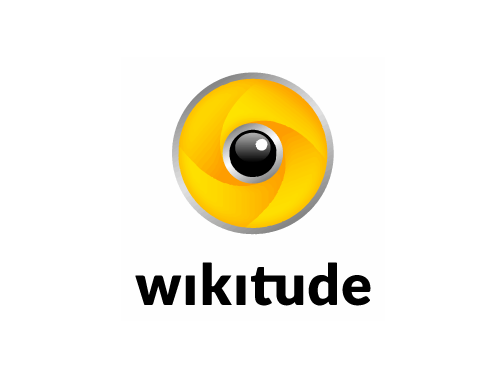
\includegraphics[width=0.2\textwidth]{Images/Wikitude_Logo.png}
    \label{fig:Wikitude}
\end{figure}
Desarrollada por Wikitude GmbH, es una de las librerías pioneras en el mundo de la realidad aumentada. Lanzaron su primera aplicación en el 2008, desde entonces, son líderes del mercado. La versión que hemos usado ha sido Wikitude SDK 8.7.0 (2019-08-13).\cite{Wikitude}
Las principales funcionalidades son:
Geo AR (Puntos de anclaje vía GPS)
Reconocimiento de imágenes 2D (marcadores) 
Reconocimiento de objetos 3D
Las plataformas móviles soportadas son:
\begin{itemize}
\item Android
\item iOS
\item Windows
\item Unity
\item Cordova
\item Xamarin
\item Flutter
\item Titanium
\end{itemize}
Soporte para Smart Glasses:
\begin{itemize}
\item Epson Moverio
\item Hololens
\item Vuzix
\end{itemize}
Otras plataformas:
\begin{itemize}
\item React Native
\item Ionic
\item Adobe Air
\item Qt by Felgo
\item LBAR
\end{itemize}
Licencias:
\begin{itemize}
\item Wikitude Demo. Licencia de 30 días con marca de agua 499€
\item Wikitude SDK PRO (Sólo con marcadores y Geo AR). 1 año de licencia 1990€
\item Wikitude SDK PRO 3D (Paquete completo). 1 año de licencia 2490€
\end{itemize}

\clearpage
\subsection{ARKit}
\begin{figure}[H]
    \centering
    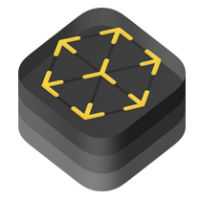
\includegraphics[width=0.2\textwidth]{Images/Arkit_Logo.jpeg}
    \label{fig:ARKit}
\end{figure} 

Desarrollado por Apple, presentado en la Apple Worldwide Developers Conference de 2017.
La versión con la que trabajamos es la ARKit SDK 3.0.\cite{AppleDeve} A diferencia del resto, para usar esta librería en Unity, no hace falta descargar ningún plugin, viene incluido en el paquete de Unity ARFoundation 2.2.
Funcionalidades:
\begin{itemize}
\item Reconocimiento de imágenes 2D (marcadores)
\item Reconocimiento de objetos 3D
\item Reconocimiento de rostro (hasta 3 simultáneamente)
\item Oclusión
\item SLAM
\item Estimación de luces
\item Puntos de anclaje en la nube
\end{itemize}
Las plataformas soportadas son:
\begin{itemize}
\item iOS 
\item Unity (via ARFoundation)
\item Unreal Engine 4.\cite{Unreal}
\end{itemize}
La licencia es gratuita.

 \clearpage
\subsection{ARCore}
 \begin{figure}[H]
    \centering
    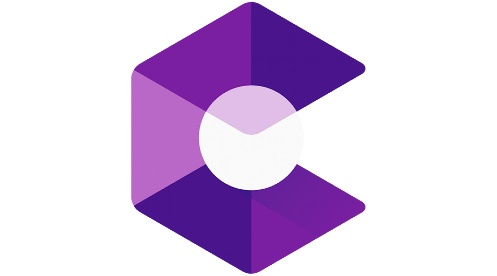
\includegraphics[width=0.2\textwidth]{Images/ARCore.jpeg}
    \label{fig:ARCore}
\end{figure}

Desarrollado por Google, fue lanzado en febrero de 2018 como respuesta para competir contra ARKit de iOS. La versión con la que trabajamos es ARCore SDK for Unity v1.11.0 (2019-05-05).\cite{ARCore}
Funcionalidades:
\begin{itemize}
\item Reconocimiento de imágenes 2D (Marcadores)
\item Reconocimiento de objetos 3D
\item Reconocimiento de rostro.
\end{itemize}
\begin{itemize}
\item SLAM
\item Mapeado de áreas grandes
\item Estimación de luces
\item Puntos de anclaje en la nube
\end{itemize}
Las plataformas soportadas son:
\begin{itemize}
\item Android
\item Android NDK
\item Unity (Android, iOS)
\item Unreal Engine 4
\item iOS
\end{itemize}
La licencia para usar ARCore es completamente gratuita.

\clearpage
\subsection{Vuforia}
\begin{figure}[H]
    \centering
    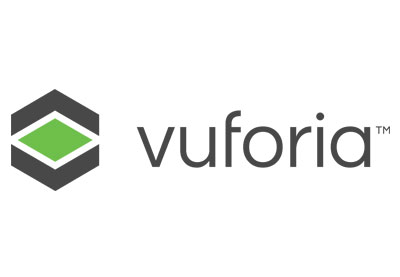
\includegraphics[width=0.2\textwidth]{Images/Vuforia.jpeg}
    \label{fig:Vuforia}
\end{figure}
Desarrollado por la empresa PTC, un proveedor tecnológico mundial de la plataforma líder de IoT (Internet of Things) y realidad aumentada. La versión que hemos utilizado ha sido Vuforia SDK Android 8.3.8 (2019-06-13).\cite{Vuforia}
Funcionalidades:
\begin{itemize}
\item Reconocimiento de imágenes 2D (Marcadores)
\item Reconocimiento de objetos 3D
\item Escáner de objetos 3D
\end{itemize}
Plataformas:
\begin{itemize}
\item Android
\item iOS
\item Windows
\item Smart Glasses
\end{itemize}
Licencias:
\begin{itemize}
\item Básica, 42\$ al mes.
\item Básica con base de datos en la nube para los marcadores 99\$ al mes.
\item Para la versión pro, la cual incluye todas las funcionalidades, hay que contactar y hacen presupuesto a medida para la empresa.
\end{itemize}

\clearpage
\subsection{Kudan}
 \begin{figure}[H]
    \centering
    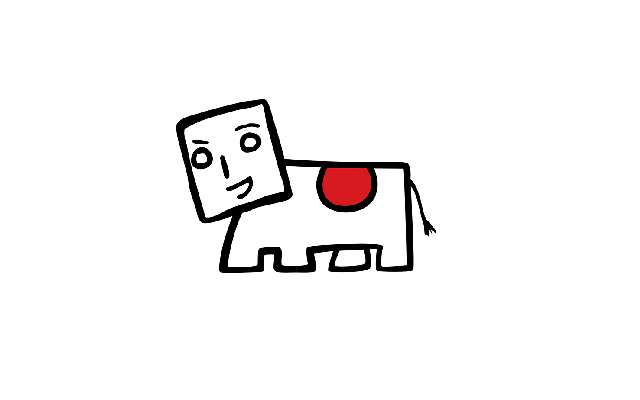
\includegraphics[width=0.2\textwidth]{Images/Kudan_Logo.png}
    \label{fig:Kudan}
\end{figure}

Kudan es una empresa que se dedica al desarrollo de la realidad aumentada, virtual y mixta, además de la conducción autónoma, drones y robots. La versión que hemos utilizado ha sido la Kudan SDK Unity 1.6.0 (2019-07-16).\cite{Kudan}
Funcionalidades:
\begin{itemize}
\item Reconocimiento de imágenes 2D (Marcadores)
\item SLAM
\end{itemize}
Plataformas:
\begin{itemize}
\item Unity (Android, iOS)
\item iOS
\item Android
\end{itemize}
Licencias:
\begin{itemize}
\item AR Indie: Gratis. Pensado para la fase de desarrollo, protegido con marca de agua.
\item AR Business: 1500\$. Para las empresas con menos de un millón de dólares en ingresos.
\item AR Enterprise: Para las empresas con más de un millón de dólares en ingresos, hay que contactar con Kudan y proporcionan un presupuesto personalizado.
\end{itemize}

\clearpage
\subsection{MaxST}

 \begin{figure}[H]
    \centering
    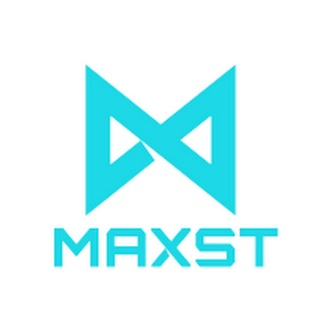
\includegraphics[width=0.2\textwidth]{Images/Maxst_Logo.jpeg}
    \label{fig:Maxst}
\end{figure}

Maxst se fundó en 2010 y se dedica a la investigación y desarrollo de la tecnología de realidad aumentada, han lanzado Maxst AR SDK, el cual hemos probado en la versión MaxstARSDK\_Unity 4.1.3. \cite{Maxst}
Funcionalidades:
\begin{itemize}
\item Reconocimiento de imágenes 2D (Marcadores)
\item Reconocimiento de objetos 3D
\item Reconocimiento de códigos de barras y QR.
\end{itemize}
Plataformas:
\begin{itemize}
\item Unity (Android,iOS)
\item Android
\item iOS
\item Windows
\item macOS
\item Epson MOVERIO BT-300,350 y ODG R-7
\end{itemize}
Licencias:

\begin{itemize}
\item Free. Gratis, para uso no comercial, incluye marca de agua.
\item Pro-one. Para aplicaciones con menos de 100k descargas (no incluye actualizaciones). Pago único de 499\$ 
\item Pro-Subscription. Subscripción anual, incluye actualizaciones 599\$ por año
\item Enterprise. Para aplicaciones con más de 100k de descargas. Hay que contactar con Maxst para recibir un presupuesto.
\end{itemize}

\clearpage
\subsection{8th Wall}
\begin{figure}[H]
    \centering
    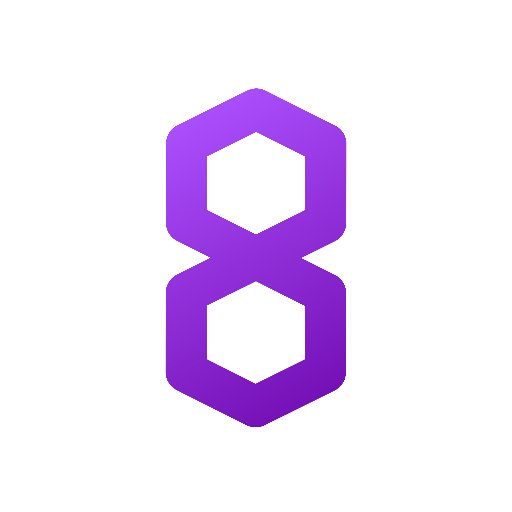
\includegraphics[width=0.2\textwidth]{Images/8thWall_Logo.jpeg}
    \label{fig:8th Wall}
\end{figure}

8th Wall desarrolla dos productos diferentes, 8th Wall Web y 8th Wall XR for Unity. El producto que vamos a analizar en este caso es el 8th Wall XR for Unity 11.2.6.519, para que la comparación entre las librerías sea mas precisa, ya que la potencia que tiene en navegador es menor a la que puede llegar a tener una aplicación de Unity. \cite{8thWall}
Funcionalidades:
\begin{itemize}
\item Reconocimiento de imágenes 2D (Marcadores)
\item 6 grados de libertad.
\item SLAM
\item Estimación de la luz
\end{itemize}

Plataformas:
\begin{itemize}
\item Unity (Android, iOS)
\item Web (A-Frame, BabylonJS, Sumerian, three.js)
\end{itemize}
El uso de 8th Wall XR de Unity es gratuito. En el caso de 8th Wall Web, la licencia se cobra según las visitas en la web. Aparte, se necesita una licencia de desarrollador que cuesta 250\$/mes.\\

\begin{center}
\begin{tabular}{| c| c |c| c |}
\hline
 Pago por visita (PPV)&	Paquete estándar&PPV de alto tráfico&Paquete alto tráfico \\
 \hline
  1000\$/mes	& 3000\$/mes	& 6000\$/mes &	6000\$/mes \\  
  \hline
 0 visitas incluidas &	500k visitas incluidas&	0 visitas incluidas	&5M visitas incluidas\\
 \hline
 0.01\$/visita&	0.01\$/visita extra&	0.0025\$/visita&	0.0025\$/visita extra\\
 \hline
\end{tabular}
\caption{Licencias 8th Wall}
\end{center}
\\

\clearpage
\subsection{Easy AR}
\begin{figure}[H]
    \centering
    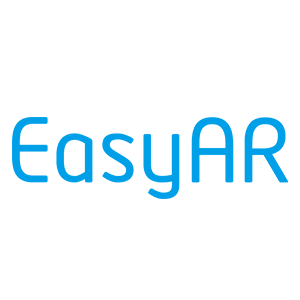
\includegraphics[width=0.2\textwidth]{Images/EasyAR.png}
    \label{fig:my_label}
\end{figure}

EasyAR es una compañía china que lleva en el mercado desde 2016. Hemos probado la versión EasyARSense Unity SDK v3.0.1(2019-07-07)\cite{EasyAR}
Funcionalidades:
\begin{itemize}
\item Reconocimiento de imágenes 2D (Marcadores)
\item Reconocimiento de objetos 3D
\item SLAM
\item Grabación de pantalla
\end{itemize}
Plataformas soportadas:
\begin{itemize}
\item Unity (Android, iOS)
\item Android
\item iOS
\item Windows
\end{itemize}
Licencias:
\begin{itemize}
\item EasyAR SDK Basic. Gratis
\item EasyAR SDK Pro. Añade el reconocimiento de objetos 3D, la grabación de pantalla y reconocimiento de más de un marcador simultáneo
\item EasyAR SDK Pro trial. Lo mismo que el Pro, pero limitado a 100 usos por día.
\end{itemize}

\clearpage
\subsection{ARFoundation}
\begin{figure}[H]
    \centering
    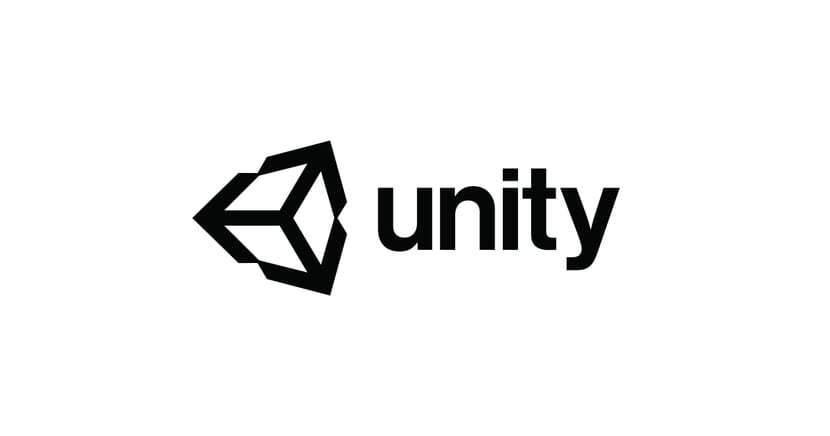
\includegraphics[width=0.2\textwidth]{Images/Unity_Logo.jpeg}
    \label{fig:my_label}
\end{figure}

Este último no se trata exactamente de una librería, es un paquete de Unity (aún en fase experimental) que integra una API de alto nivel (wrapper) que permite tener el mismo código funcional para ARCore y ARKit, según si exportamos el proyecto en Android o en iOS. La versión más reciente es ARFoundation 2.2 (Unity 2019.1), la cual incluye ARKit 3.\cite{ARFoundation}\\
Soporta las mismas funcionalidades que ARCore y ARKit:
\begin{itemize}
\item Reconocimiento de imágenes 2D (marcadores)
\item Reconocimiento de objetos 3D.
\item Reconocimiento de rostro 
\item Oclusión (iOS con ARKit)
\item SLAM
\item Mapeado de áreas grandes (ARCore)
\item Estimación de luces
\item Puntos de anclaje en la nube
\end{itemize}

Plataformas soportadas:
\begin{itemize}
\item Unity (Android, iOS)
\end{itemize}

Su licencia, al igual que ARCore y ARKit, es gratuita.

\noindent